\RequirePackage[l2tabu, orthodox]{nag}
\documentclass{article} % Angiver skriftstørrelse og dokumenttype
\usepackage[top=1cm, bottom=0.5cm, left=0cm, right=1cm]{geometry}
\usepackage{graphicx} % Importerer figurer
\usepackage{wrapfig} % Placerer figurer
\usepackage{microtype} % Bedre typografi
\usepackage{amsmath} % Bedre matematik
\usepackage[utf8]{inputenc} % Tillader danske tegn
\usepackage[english]{babel} % Angiver sprog. Udskift evt. med "Danish"
\usepackage{datetime}
\usepackage{booktabs}
\usepackage{cmbright}
\usepackage[T1]{fontenc}
\usepackage{epstopdf}
\usepackage{fancyhdr}
\usepackage[table]{xcolor}

\begin{document}
\pagestyle{empty}
\begin{tabular}{b{0.30\paperwidth}b{0.30\paperwidth}b{0.30\paperwidth}}
	\rowcolor{gray}	& 	& \\[4ex]
  	\rowcolor{gray} \multicolumn{2}{l}{\hspace{1cm} \textcolor{white}{\Large \textbf{ProjektFormidlingNord}}} & \\[5ex]	
  	&&\\
\begin{tabular}{r|c}
  	Net Asset Value & 100.000.000 \\
  	No. of Assets & 42 \\
  	Avg. Pos & 100.000 \\
  	Portfolio vol. & 8\% \\
  	Mean return & 10\% \\
  	Beta & 1.2 \\
\end{tabular} & \multicolumn{2}{l}{\raisebox{-0.5\height}{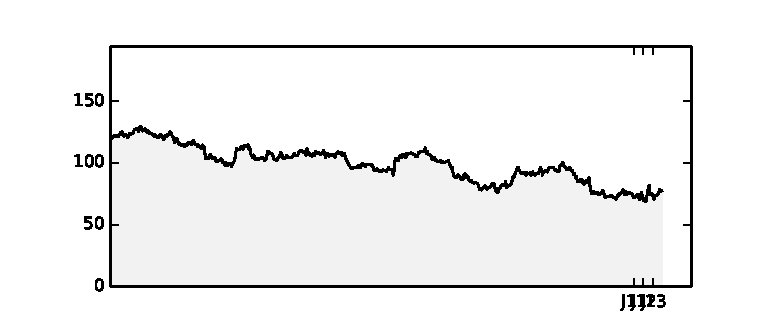
\includegraphics[]{nav.eps}}} \\
&& \\
\begin{tabular}{lr}

\toprule

Monthly value movers\\
\midrule

GN Store Nord & 78,788\\
China Gas Holdings & 30,568\\
Carlsberg & 23,326\\
\midrule

Lundbeck & -9,999\\
D/S Norden & -11,179\\
East asian company & -11,357\\
\bottomrule

\end{tabular} & \begin{tabular}{lr}

\toprule

Monthly percentage movers\\
\midrule

Topo Target & 16.33\%\\
Vestas & 13.63\%\\
TK Development & 12.58\%\\
\midrule

Lundbeck & -11.21\%\\
Genmab & -12.81\%\\
East asian company & -15.20\%\\
\bottomrule

\end{tabular} & {\raisebox{-0.5\height}{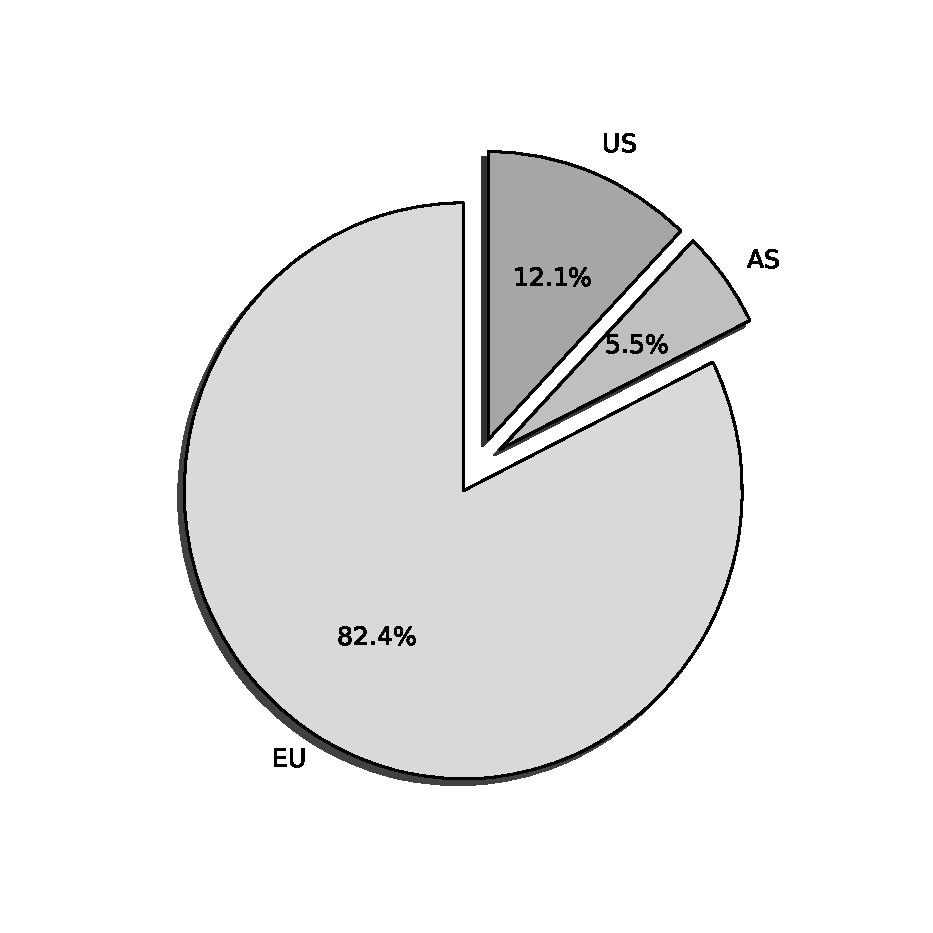
\includegraphics[width=0.3\textwidth]{pie.eps}}}
\end{tabular} 

\pagebreak{}

\begin{tabular}{b{0.30\paperwidth}b{0.30\paperwidth}b{0.30\paperwidth}}
	\rowcolor{gray}	& 	& \\[4ex]
  	\rowcolor{gray} \multicolumn{2}{l}{\hspace{1cm} \textcolor{white}{\Large \textbf{ProjektFormidlingNord}}} & \\[5ex]	
  	&&\\
\multicolumn{3}{c}{\begin{tabular}{lrrrrrrrrr}

Asset & Price & Holding & NaV & YoY\% & MoM\% & Div. Yield & Sector & Region & Beta \\

GN Store Nord & 64.65 & 11,579 & \bf{748,582} & -26.53\% & -10.21\% & 0.00\% & Healthcare & EU & B\\
Carlsberg & 484.3 & 1,014 & \bf{491,080} & -15.48\% & 13.37\% & 0.00\% & Forbrugsvarer & EU & B\\
Danske Bank & 83.3 & 4,343 & \bf{361,771} & -23.01\% & 0.18\% & 0.00\% & Finans & EU & B\\
FL Schmidt & 348.4 & 876 & \bf{305,198} & -1.58\% & 11.06\% & 0.00\% & Industri & EU & B\\
Novozymes & 152.2 & 1,135 & \bf{172,747} & -11.51\% & -5.7\% & 0.00\% & Healthcare & EU & B\\
East asian company & 146.0 & 874 & \bf{127,604} & 28.63\% & 5.8\% & 0.00\% & Forbrugsvarer & EU & B\\
China Gas Holdings & 3.85 & 30,000 & \bf{115,500} & -44.28\% & 6.94\% & 0.00\% & Forsyning & A & B\\
Shenhua Energy & 30.7 & 3,500 & \bf{107,450} & -7.39\% & 18.3\% & 0.00\% & Materialer & A & B\\
Ericsson & 61.45 & 1,630 & \bf{100,163} & -8.49\% & -0.41\% & 0.00\% & Teknologi & EU & B\\
Hennes and Mauritz & 224.6 & 400 & \bf{89,840} & -1.88\% & 4.17\% & 0.00\% & Cyklisk forbrug & EU & B\\
Nordea & 45.69 & 1,627 & \bf{74,337} & -19.49\% & -1.76\% & 0.00\% & Finans & EU & B\\
D/S Norden & 151.4 & 480 & \bf{72,672} & -11.41\% & -4.6\% & 0.00\% & Industri & EU & B\\
NKT Holding & 229.3 & 282 & \bf{64,662} & 16.75\% & 13.35\% & 0.00\% & Teknologi & EU & B\\
Lundbeck & 118.6 & 518 & \bf{61,434} & 34.77\% & -4.43\% & 0.00\% & Healthcare & EU & B\\
Statoil & 25.23 & 2,285 & \bf{57,650} & -99.73\% & 12.23\% & 0.00\% & Olie og Gas & EU & B\\
Maersk & 7976.0 & 7 & \bf{55,832} & -15.58\% & 6.86\% & 0.00\% & Industri & US & B\\
Novo Nordisk & 142.29 & 339 & \bf{48,236} & -98.49\% & 5.98\% & 0.00\% & Healthcare & EU & B\\
Bavarian Nordic & 44.1 & 786 & \bf{34,662} & -10.37\% & -10.18\% & 0.00\% & Healthcare & EU & B\\
Procter and Gamble & 63.58 & 434 & \bf{27,593} & 8.87\% & 1.66\% & 0.00\% & Forbrugsvarer & US & B\\
Alk-Abello & 388.0 & 67 & \bf{25,996} & -5.71\% & 8.38\% & 0.00\% & Healthcare & EU & B\\
TK Development & 14.3 & 1,786 & \bf{25,539} & 13.49\% & 1.42\% & 0.00\% & Ejendomme & EU & B\\
SAP AG & 48.81 & 460 & \bf{22,452} & -16.42\% & 5.6\% & 0.00\% & Teknologi & EU & B\\
Vestas & 42.12 & 422 & \bf{17,774} & 9.97\% & 37.92\% & 0.00\% & Industri & EU & B\\
Microsoft & 30.68 & 560 & \bf{17,180} & -45.94\% & 6.16\% & 0.00\% & Teknologi & US & B\\
Teva Phama & 40.67 & 420 & \bf{17,081} & -76.2\% & 4.44\% & 0.00\% & Healthcare & US & B\\
Topo Target & 2.99 & 4,800 & \bf{14,352} & 30.57\% & -13.58\% & 0.00\% & Healthcare & EU & B\\
Wal-Mart & 59.07 & 229 & \bf{13,527} & -65.44\% & -12.53\% & 0.00\% & Cyklisk forbrug & US & B\\
Johnson and Johnson & 63.93 & 196 & \bf{12,530} & 9.47\% & 2.91\% & 0.00\% & Healthcare & US & B\\
Genmab & 41.25 & 250 & \bf{10,312} & -56.62\% & -4.4\% & 0.00\% & Healthcare & EU & B\\
Citigroup Inc. & 28.14 & 365 & \bf{10,271} & -51.82\% & 6.27\% & 0.00\% & Finans & US & B\\
Neurosearch & 9.75 & 407 & \bf{3,968} & 172.35\% & 148.72\% & 0.00\% & Healthcare & EU & B\\
Torm & 1.98 & 1,246 & \bf{2,467} & 11.24\% & -15.02\% & 0.00\% & Industri & EU & B\\
\end{tabular}}
\end{tabular} 
\end{document}